%-----------------------------------------------------------------------------%
\chapter{\topikTiga}
%-----------------------------------------------------------------------------%

%-----------------------------------------------------------------------------%
\section{Pendahuluan}
%-----------------------------------------------------------------------------%
	Conjugate gradient method digunakan untuk menyelesaikan persamaan linear $Ax = b$ di mana matriks koefisiennya bersifat simetris dan definit positif.  Matriks $A$ $n$ x $n$ dikatakan simetris jika $a_{ij}$ = $a_{ji}$ untuk $i,j = 1,...,n$.  Matriks $A$ dikatakan definit positif jika untuk setiap vektor $x$ bukan nol, perkalian skalar $x \cdot Ax$ menghasilkan nilai lebih besar dari nol.
	Algoritma conjugate gradient method ditunjukkan pada \pic~\ref{fig:cg}.  $r_{k}$ merupakan sisa atau selisih antara $b$ 
	dengan $Ax_{k}$, sedangkan $p_{k}$ merupakan \f{search direction}.
	
	\begin{figure}
		\centering
		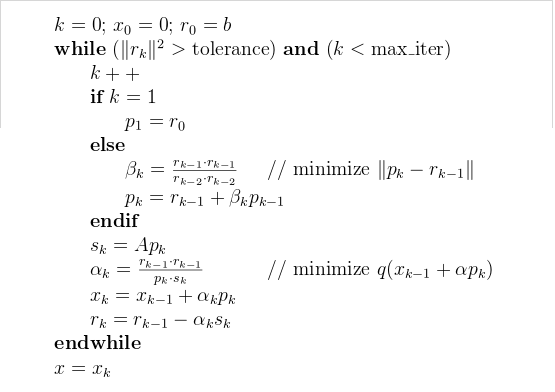
\includegraphics[width=0.75\textwidth]
			{pics/cg_par.png}
		\caption{Algoritma Conjugate Gradient Method.}
		\label{fig:cg}
	\end{figure}  
	
	Pada implementasi paralel CGM, matriks $A$ akan didistribusikan menggunakan fungsi \texttt{MPI\_scatter} kepada setiap proses dan masing-masing proses mendapat sebanyak $n$ x $n$ / $p$ data.  Algoritma tersebut dijalankan di setiap proses untuk setiap bagian distribusi matriks $A$.
%-----------------------------------------------------------------------------%
\section{Eksperimen}
%-----------------------------------------------------------------------------%

	Implementasi algoritma paralel CGM menggunakan kode sumber yang dibangun oleh Joseph Tanigawa yang dipublikasikan melalui Github.  Eksperimen dilakukan di lingkungan cluster Fasilkom dan nbcr-233.ucsd.edu.  Percobaan dilakukan dengan variasi jumlah prosesor dan besar data.  Banyaknya prosesor yang digunakan mulai dari 2 sampai dengan 8 sedangkan besar data yang digunakan adalah 512, 1024, dan 2048.  \pic~\ref{fig:cgfasilkom} dan \pic~\ref{fig:cgnbcr} berturut-turut menunjukkan hasil unjuk kerja implementasi algoritma paralel CGM di cluster Fasilkom dan nbcr-233.ucsd.edu.  Pada grafik tersebut menunjukkan \f{execution time} per iterasi karena setiap eksperimen menghasilkan jumlah iterasi yang berbeda-beda.  Pada eksperimen tersebut kami atur jumlah maksimum iterasi yang diijinkan adalah 1000 dengan toleransi ($r$) sebesar 1e-06.
	
	\begin{figure}
		\centering
		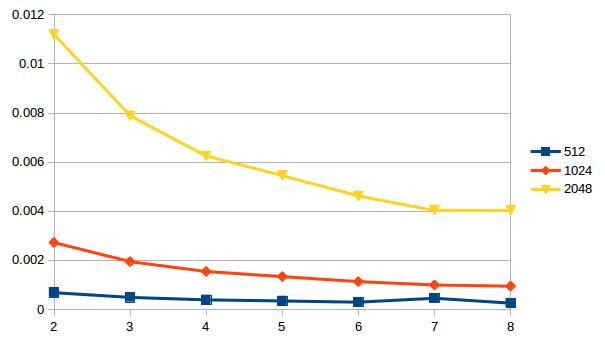
\includegraphics[width=0.8\textwidth]
			{pics/cg_fasilkom.jpg}
		\caption{Hasil eksperimen paralel CG pada cluster Fasilkom.}
		\label{fig:cgfasilkom}
	\end{figure}
		
	\begin{figure}
		\centering
		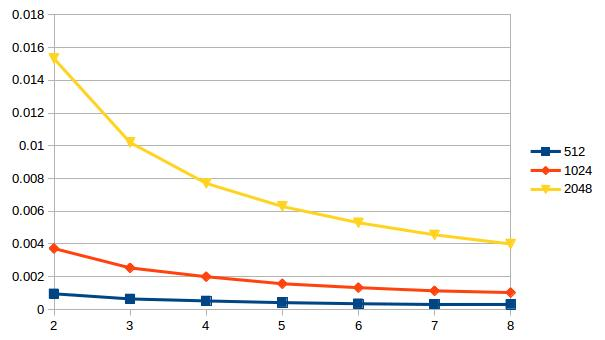
\includegraphics[width=0.8\textwidth]
			{pics/cg_nbcr.jpg}
		\caption{Hasil eksperimen paralel CG pada cluster nbcr-233.ucsd.edu.}
		\label{fig:cgnbcr}
	\end{figure}
	
	Dari grafik tersebut menunjukkan bahwa paralelisasi algoritma CGM menghasilkan \f{speed up}.  Meski terdapat penyimpangan saat melakukan eksperimen di cluster Fasilkom namun secara keseluruhan terdapat peningkatan performa.